\section{Bias Variance Decomposition}  

  The likelihood defines a proper loss function. Now let's try to parse the loss a bit more. It turns out that for a lot of popular loss functions, they generally decomposes into 
  \begin{equation}
    \text{Loss} = \text{Bias} + \text{Variance} + \text{Noise}
  \end{equation} 

  This decomposition is by no means exact, but it \textit{generally} holds true. This is formalized by deriving an exact decomposition of the MSE loss. This is possible because the MSE loss allows us to get an $L^2$ space, which allows for orthogonal decompositions. Unfortunately, when you have other losses, this becomes much messier because the inner product structure is not there. 

  In a more general case, when you take a supremum of risk over a function class, it decomposes into 3 terms. 
  \begin{enumerate}
    \item One of which quantifies how big the function class is (more variance). 
    \item One of which quantifies the distance between the truth and the function class (bias).  
    \item One is the noise term, which is the irreducible error. 
  \end{enumerate}

  \begin{example}[Bias and Variance Tradeoff in Polynomial Regression]
    Let's motivate this by trying to fit a polynomial on some data. 
    \begin{figure}[H]
      \centering 
      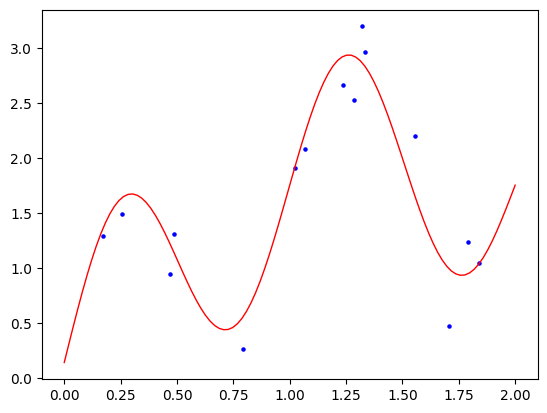
\includegraphics[scale=0.4]{img/True_data.png}
      \caption{A sample of $|\mathcal{D}| = 15$ data points are generated from the function $f(x) = \sin(2\pi x) + 2\cos (x - 1.5)$ with Gaussian noise $N(0, 0.3)$ on the interval $[0, 1]$. } 
      \label{fig:true_data}
    \end{figure}

    If we try to fit a polynomial function, how do we know which degree is best? Well the most simple thing is to just try all of them. To demonstrate this even further, I generated 10 different datasets  $\mathcal{D}$ of size $15$ taken from the same true distribution. The best fitted polynomials for each dataset is shown below. 

    \begin{figure}[H]
      \centering 
      \begin{subfigure}[b]{0.32\textwidth}
      \centering
        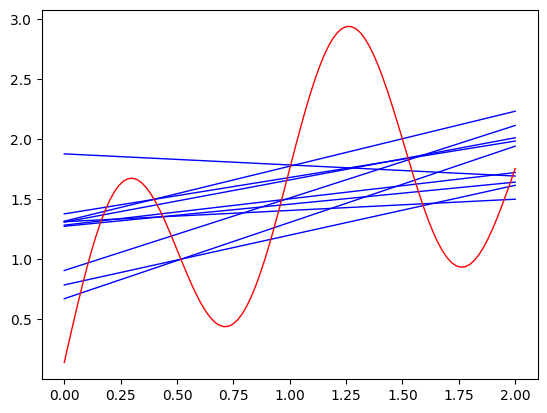
\includegraphics[width=\textwidth]{img/poly_1_fit.png}
        \caption{1st Degree}
        \label{fig:1d}
      \end{subfigure}
      \hfill 
      \begin{subfigure}[b]{0.32\textwidth}
      \centering
        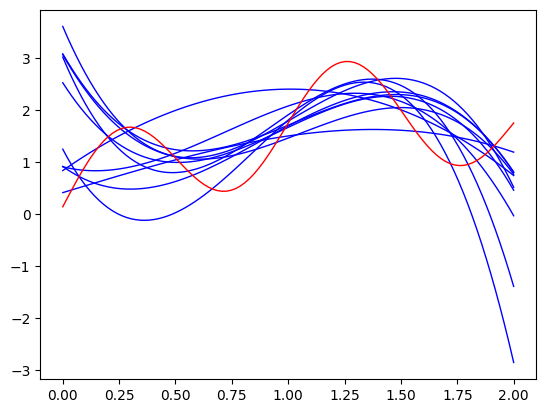
\includegraphics[width=\textwidth]{img/poly_3_fit.png}
        \caption{3rd Degree}
        \label{fig:3d}
      \end{subfigure}
      \hfill 
      \begin{subfigure}[b]{0.32\textwidth}
      \centering
        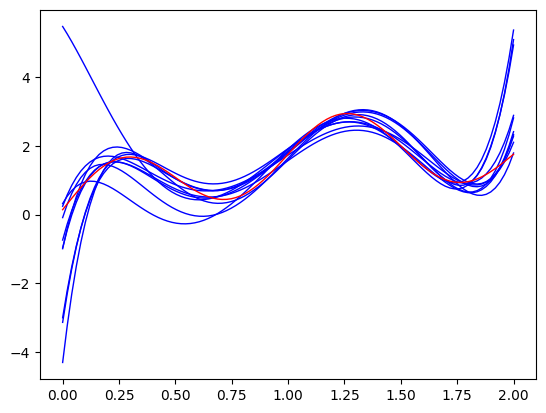
\includegraphics[width=\textwidth]{img/poly_5_fit.png}
        \caption{5th Degree}
        \label{fig:5e}
      \end{subfigure}

      \begin{subfigure}[b]{0.32\textwidth}
      \centering
        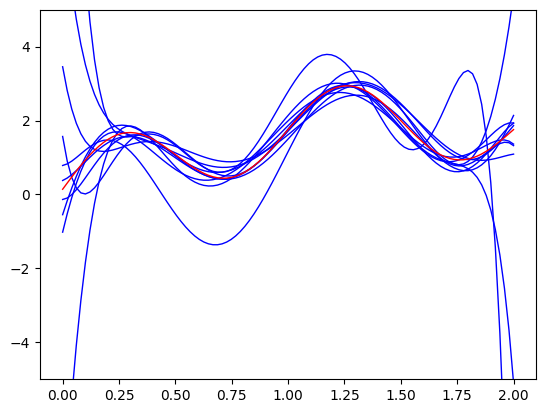
\includegraphics[width=\textwidth]{img/poly_7_fit.png}
        \caption{7th Degree}
        \label{fig:7d}
      \end{subfigure}
      \hfill 
      \begin{subfigure}[b]{0.32\textwidth}
      \centering
        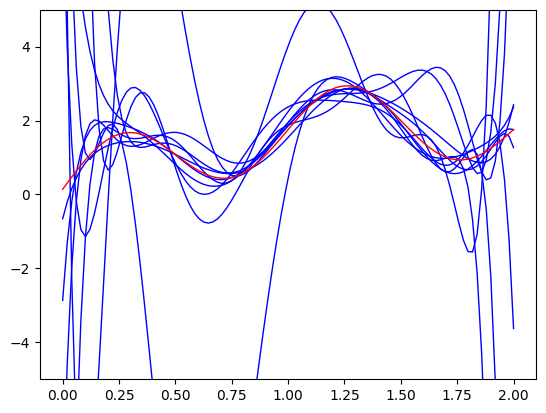
\includegraphics[width=\textwidth]{img/poly_9_fit.png}
        \caption{9th Degree}
        \label{fig:9d}
      \end{subfigure}
      \hfill 
      \begin{subfigure}[b]{0.32\textwidth}
      \centering
        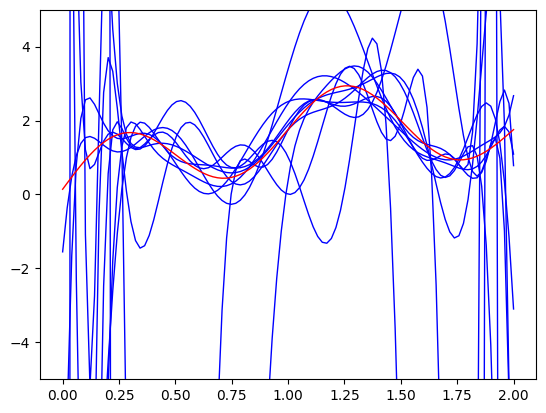
\includegraphics[width=\textwidth]{img/poly_11_fit.png}
        \caption{11th Degree}
        \label{fig:11e}
      \end{subfigure}

      \caption{Different model complexities (i.e. different polynomial degrees) lead to different fits of the data generated from the true distribution. The lower degree best fit polynomials don't have much variability in their best fits but have high bias, while the higher degree best fit polynomials have very high variability in their best fits but have low bias. The code used to generate this data is \href{code/polynomial_fitting.ipynb}{here}. }
      \label{fig:polynomial_fitting}
    \end{figure}

    We already know that the 5th degree approximation is most optimal, and the lower degree ones are \textbf{underfitting} the data, while the higher degree ones are \textbf{overfitting}. As mentioned before, we can describe the underfitting and overfitting phenomena through the bias variance decomposition. 

    \begin{enumerate}
      \item If we underfit the data, this means that our model is not robust and does not capture the patterns inherent in the data. It has a high bias since the set of function it encapsulates is not large enough to model $\mathbb{E}[Y\mid X]$. However, it has a low variance since if we were to take different samples of the dataset $\mathcal{D}$, the optimal parameters would not fluctuate. 

      \item What overfitting essentially means is that our model is too complex to the point where it starts to fit to the \textit{noise} of the data. This means that the variance is high, since different samples of the dataset $\mathcal{D}$ would cause huge fluctuations in the optimal trained parameters $\boldsymbol{\theta}$. However, the function set would be large, and thus it would be close to $\mathbb{E}[Y \mid X]$, leading to a low bias. 
    \end{enumerate}
  \end{example}
  
  \begin{example}[Polynomial Regression Continued]
    Another way to reduce the overfitting problem is if we have more training data to work with. That is, if we were to fit a 9th degree polynomial on a training set of not $N = 15$, but $N = 100$ data points, then we can see that this gives a much better fit. This makes sense because now the random variable $\mathcal{D}$, as a function of more random variables, has lower variance. Therefore, the lower variance in the dataset translates to lower variance in the optimal parameter. 

    \begin{figure}[H]
      \centering
      \begin{subfigure}[b]{0.48\textwidth}
      \centering
        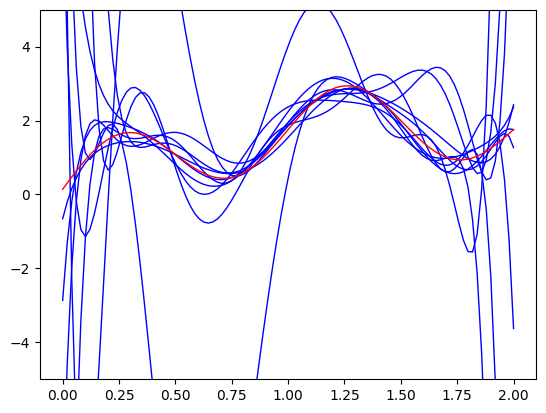
\includegraphics[width=\textwidth]{img/poly_9_fit.png}
        \caption{$M = 9, N = 15$}
        \label{fig:less_points}
      \end{subfigure}
      \hfill 
      \begin{subfigure}[b]{0.48\textwidth}
      \centering
        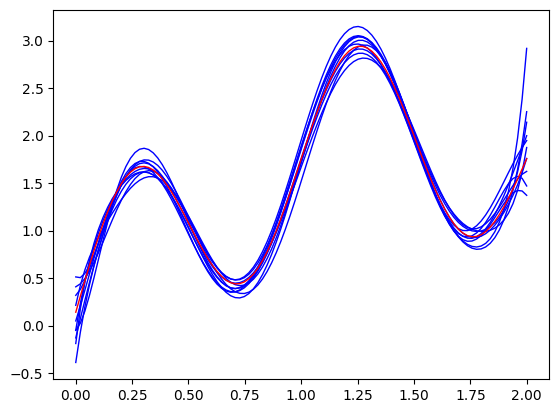
\includegraphics[width=\textwidth]{img/increased_data.png}
        \caption{$M = 9, N = 100$}
        \label{fig:more_points}
      \end{subfigure}
      \caption{Increasing the number of data points helps the overfitting problem. Now, we can afford to fit a 9th degree polynomial with reasonable accuracy.}
      \label{fig:reducing_overfitting_with_more_samples}
    \end{figure}
  \end{example}



\subsection{MSE Loss} 

  \begin{definition}[Mean Squared Error Loss]
    \label{mse_loss}
    The \textbf{MSE loss} is defined 
    \begin{equation}
      L(y, x) = (y - f(x))^2
    \end{equation}
  \end{definition}

  It is a well known fact that the true regressor---which may not be linear at all---that minimizes this loss is 
  \begin{equation}
    f^\ast (x) = \mathbb{E}[Y \mid X = x]
  \end{equation}
  which is the conditional expectation of $Y$ given $X$. This is the true regressor function, which is the best approximation of $Y$ over the $\sigma$-algebra generated by $X$. Therefore, if we consider a function class of linear predictors, we can decompose our risk, which is the distance between our estimated linear regressor and $Y$, as the sum of the distance between our estimator and the best regressor plus the distance between the best regressor and $Y$. 

  \begin{theorem}[Pythagorean's Theorem]
    The expected square loss over the joint measure $\mathbb{P}_{x, y}$ can be decomposed as 
    \begin{equation}
      \mathbb{E}_{x, y} [( y - f(x))^2] = \mathbb{E}_{x, y} [\big(y - \mathbb{E}[y \mid x]\big)^2] + \mathbb{E}_x [\big(\mathbb{E}[y \mid x] - h(x) \big)^2]
    \end{equation}
    That is, the squared loss decomposes into the squared loss of $\mathbb{E}[y \mid x]$ and $g(x)$, which is the intrinsic misspecification of the model, plus the squared difference of $y$ with its best approximation $\mathbb{E}[y \mid x]$, which is the intrinsic noise inherent in $y$ beyond the $\sigma$-algebra of $x$. 
  \end{theorem}
  \begin{proof}
    We can write 
    \begin{align}
      \mathbb{E}_{x, y} \big[ \big(y - f(x)\big)^2 \big] & = \mathbb{E}_{x, y}\big[ \big((y - \mathbb{E}[y \mid x]) + (\mathbb{E}[y \mid x] - f(x)) \big)^2 \big] \\
      & = \mathbb{E}_{x, y} [\big(y - \mathbb{E}[y \mid x]\big)^2] + \mathbb{E}_{x, y} [\{y - \mathbb{E} [y \mid x]\} \, \{ \mathbb{E}[y \mid x] - f(x) \}] \\
      & \;\;\;\;\;\;\;\;\;\;\;\;\;\;\; + \mathbb{E}_x [\big(\mathbb{E}[y \mid x] - f(x) \big)^2] \\
      & = \mathbb{E}_{x, y} [\big(y - \mathbb{E}[y \mid x]\big)^2] + \mathbb{E}_x [\big(\mathbb{E}[y \mid x] - f(x) \big)^2]
    \end{align}
    where the middle term cancels out due to the tower property. 
  \end{proof}

  Note that since $\mathbb{E}[\big(\mathbb{E}[Y \mid X] - g(X) \big)^2]$ is the misspecification of the model, we cannot change this (positive) constant, so $\mathbb{E}\big[ \big(Y - g(X)\big)^2 \big] \geq \mathbb{E}[(Y - \mathbb{E}[Y \mid X])^2]$, with equality achieved when we perfectly fit $g$ as $\mathbb{E}[Y \mid X]$ (i.e. the model is well-specified). Therefore, denoting $\mathcal{F}$ as the set of all $\sigma(X)$-measurable functions, then the minimum of the loss is attained when 
  \begin{equation}
    \argmin_{g \in \mathcal{F}} \mathbb{E}[L] = \argmin_{g \in \mathcal{F}} \mathbb{E} \big[ \big(Y - g(X)\big)^2 \big] = \mathbb{E}[Y \mid X]
  \end{equation}
  Essentially, we have decomposed our risk to a part that we can optimize and a part that we cannot, i.e. the intrinsic noise. 

  \begin{corollary}[Sufficient to Estimate Conditional Expectation]
    Minimizing the prediction risk is equivalent to minimizing the risk of our estimator to the conditional distribution. 
    \begin{equation}
      \argmin_{f \in \mathcal{F}} R(f) = \argmin_{f \in \mathcal{F}} \mathbb{E}_{x, y} \left[ (\mathbb{E}[y|x] - f(x))^2 \right]
    \end{equation}
  \end{corollary}
  
  Even though this example is specific for the mean squared loss, this same decomposition, along with the bias variance decomposition, exists for other losses. It just happens so that the derivations are simple for the MSE, which is why this is introduced first. However, the derivations for other losses are much more messy, and sometimes may not hold rigorously. However, the general intuition that more complex models tend to overfit (higher variance) still hold true. 

  Let's try to decompose this even more. In frequentist inference, we take a dataset $\mathcal{D}$ and optimize $\hat{f}$ that minimizes this empirical risk. Therefore, for a given $\mathcal{D}$, $\hat{f} = \hat{f}(\mathcal{D})$ is determined, and if $\mathcal{D} = (x^{(i)}, y^{(i)})^n$ is a random variable, then $\hat{f}$ is also a random variable, which we will denote as $\hat{f}_{\mathcal{D}}$ for clarity. It is useful to think of $\mathcal{D}$ as a random variable because by seeing how $\hat{f}_{\mathcal{D}}$ varies as the dataset changes, we can measure the uncertainty in our estimate of $\hat{f}_{\mathcal{D}}$ through $\mathcal{D}$.\footnote{If this didn't make sense to you, consider the following thought experiment. Suppose we had a large number of datasets each of size $N$ and each drawn independently from the joint distribution $X \times Y$. For any given dataset $\mathcal{D}$, we can run our learning algorithm and obtain our best fit function $\hat{f}_{\mathcal{D}}$. Different datasets from the ensemble will give different functions and consequently different values of the squared loss. }

  \begin{lemma}[Conditional Prediction Risk] 
    Our conditional prediction risk is 
    \begin{equation}
      r(\mathcal{D}) = \mathbb{E}_{x, y} \left[ (\mathbb{E}[y \mid x] - \hat{f}(x))^2 \mid \mathcal{D} \right]
    \end{equation}
    If $\mathcal{D}$ is fixed, then this is a real number. If $\mathcal{D}$ is a random variable, then this is a real-valued random variable. 
  \end{lemma} 

  Ideally, we would like two things. 
  \begin{enumerate}
    \item \textit{Low Bias}. The average prediction we get over all $\hat{f}_{\mathcal{D}}$ trained on all possible samples of dataset $\mathcal{D}$ should be similar to our best regressor. That is, 
    \begin{equation}
      \mathbb{E}_{\mathcal{D}} \left[ \mathbb{E}_{x, y} \left[ (\mathbb{E}[y \mid x] - \hat{f}_{\mathcal{D}}(x))^2 \right] \right]
    \end{equation}
    should be as low as possible. 

    \item \textit{Low Variance}. The variance of our conditional prediction risk  
    \begin{equation}
      \Var_{\mathcal{D}} \left[ \mathbb{E}_{x, y} \left[ (\mathbb{E}[y \mid x] - \hat{f}_{\mathcal{D}}(x))^2 \right] \right]
    \end{equation}
    should be as low as possible. That is, we may get very low bias for one dataset $\mathcal{D}$, but if we sampled a different dataset, we should not expect the bias to explode. 
  \end{enumerate}

  Unfortunately, having both low bias \textit{and} low variance is not possible, and we wish to show that now. 

  \begin{theorem}[Bias Variance Decomposition Under MSE Loss]
    The expected optimal MSE loss decomposes to 
    \begin{equation}
      \mathbb{E}_{\mathcal{D}} \left[ (\mathbb{E}[y \mid x] - \hat{f}_\mathcal{D} (x))^2 \right] = \underbrace{ \big( \mathbb{E}[y \mid x] - \mathbb{E}_{\mathcal{D}} [\hat{f}_\mathcal{D} (x)] \big)^2}_{(\text{bias of } \hat{f}_{\mathcal{D}})^2} + \underbrace{ \mathbb{E}_\mathcal{D} \big[ \big( \mathbb{E}_\mathcal{D} [\hat{f}_\mathcal{D} (x)] - \hat{f}_\mathcal{D} (x) \big)^2 \big]}_{\text{variance of } \hat{f}_{\mathcal{D}}}
    \end{equation}
  \end{theorem}
  \begin{proof}
    Consider the term $\big(\mathbb{E}[y \mid x] - \hat{f}_{\mathcal{D}}(x) \big)^2$ above, which models the discrepancy in our optimized hypothesis and the best approximation. We take $\mathbb{E}_{\mathcal{D}} [ \hat{f}_{\mathcal{D}} (x)]$\footnote{Over all datasets $\mathcal{D}$, there will be a function $h_{{\boldsymbol{\theta}}; \mathcal{D}}$, and averaged over all datasets $\mathcal{D}$ is $\mathbb{E}_\mathcal{D} [ \hat{f}_{\mathcal{D}}]$. } So we can split the term into 

    \begin{align}
      \big(\mathbb{E}[y \mid x] - \hat{f}_{\mathcal{D}} (x) \big)^2 & =  \big[ \big( \mathbb{E}[y \mid x] - \mathbb{E}_\mathcal{D} [\hat{f}_{\mathcal{D}} (x)] \big) + \big( \mathbb{E}_\mathcal{D} [\hat{f}_{\mathcal{D}} (x)] - \hat{f}_{\mathcal{D}} (x) \big) \big]^2 \\
      & = \big( \mathbb{E}[y \mid x] - \mathbb{E}_\mathcal{D} [\hat{f}_{\mathcal{D}} (x)] \big)^2 + \big( \mathbb{E}_\mathcal{D} [\hat{f}_{\mathcal{D}} (x)] - \hat{f}_{\mathcal{D}} (x) \big)^2 \\
      & \;\;\;\;\;\;\;\; + 2 \big( \mathbb{E}[y \mid x] - \mathbb{E}_\mathcal{D} [\hat{f}_{\mathcal{D}} (x)] \big) \big( \mathbb{E}_\mathcal{D} [\hat{f}_{\mathcal{D}} (x)] - \hat{f}_{\mathcal{D}} (x) \big) 
    \end{align}

    Now take the expectation over $\mathcal{D}$, and for the third term, note that $\big( \mathbb{E}[y \mid x] - \mathbb{E}_\mathcal{D} [\hat{f}_{\mathcal{D}} (x)] \big)$ is constant with respect to $\mathbb{D}$ anyways, so we can take it out of the expectation. Therefore, 
    \begin{align}
      \mathbb{E}_{\mathcal{D}} \big[ \big( \mathbb{E}[y \mid x] - & \mathbb{E}_\mathcal{D} [\hat{f}_{\mathcal{D}} (x)] \big) \big( \mathbb{E}_\mathcal{D} [\hat{f}_{\mathcal{D}} (x)] - \hat{f}_{\mathcal{D}} (x) \big) \big] \\
      & = \big( \mathbb{E}[y \mid x] - \mathbb{E}_\mathcal{D} [\hat{f}_{\mathcal{D}} (x)] \big) \, \mathbb{E}_{\mathcal{D}} \big[ \mathbb{E}_\mathcal{D} [\hat{f}_{\mathcal{D}} (x)] - \hat{f}_{\mathcal{D}} (x) \big] \\ 
      & = \big( \mathbb{E}[y \mid x] - \mathbb{E}_\mathcal{D} [\hat{f}_{\mathcal{D}} (x)] \big) \cdot 0 = 0
    \end{align} 
  \end{proof} 

  Let's parse these terms a bit more. 
  \begin{enumerate}
    \item The bias $\mathbb{E}[y \mid x] - \mathbb{E}_{\mathcal{D}} [\hat{f}_\mathcal{D} (x)]$ is a random variable of $x$ that measures the difference between the average of our learned predictor $\mathbb{E}_{\mathcal{D}} [\hat{f}_\mathcal{D} (x)]$ and the true regressor $\mathbb{E}[y \mid x]$. 

    \item The variance $\mathbb{E}_\mathcal{D} \big[ \big( \mathbb{E}_\mathcal{D} [\hat{f}_\mathcal{D} (x)] - \hat{f}_\mathcal{D} (x) \big)^2 \big]$ is a random variable of $x$ that measures the variability of our learned functions $\hat{f}_{\mathcal{D}}$ around our mean $\mathbb{E}_\mathcal{D} [\hat{f}_\mathcal{D} (x)]$. 
  \end{enumerate}

  Therefore, we can substitute this back into our Pythagoras decomposition, where we must now take the expected bias and the expected variance over $x$ to get a form like 
  \begin{equation}
    \text{Expected Loss} = (\text{Expected Bias})^2 + \text{Expected Variance} + \text{Noise}
  \end{equation}

  \begin{corollary}[Bias Variance Decomposition of Expected MSE Loss] 
    \label{bias_variance_mse}
    The expected optimal MSE loss decomposes to 
    \begin{align}
      \mathbb{E}_{\mathcal{D}} \mathbb{E}_{x, y} \big[ (y - \hat{f}_{\mathcal{D}}(x))^2 \big] 
      & = \mathbb{E}_{x} \big[ \underbrace{ \big( \mathbb{E}[y \mid x] - \mathbb{E}_{\mathcal{D}} [\hat{f}_\mathcal{D} (x)] \big)^2}_{\text{(expected bias)}^2} \big] + \underbrace{ \mathbb{E}_\mathcal{D} \big[ \mathbb{E}_{x} \big[ \big( \mathbb{E}_\mathcal{D} [\hat{f}_\mathcal{D} (x)] - \hat{f}_\mathcal{D} (x) \big)^2 \big] \big]}_{\text{expected variance}} \\ 
      & \;\;\;\;\;\;\;\;\;\;\;\;\;\;\;\;\;\;\;\;\;\;\;\;\; + \underbrace{\mathbb{E}_{x, y} [(y - \mathbb{E}[y \mid x])^2]}_{\text{noise}}
    \end{align}
  \end{corollary}
  \begin{proof}
    By taking the expectation over $x$ and swapping the expectations (since $x$ and $\mathcal{D}$ are independent), and finally substituting back to Pythagoras decomposition, we get the following. 
  \end{proof}
  
\subsection{MAE Loss} 

  

